\documentclass{beamer}

%\usefonttheme{professionalfonts} % using non standard fonts for beamer
%\usefonttheme{serif} % default family is serif
%\usepackage{fontspec}
%\setmainfont{Liberation Serif} %Compile XeLaTeX

\mode<presentation> {
\usetheme{Malmoe} 
\usecolortheme{beaver} 
}

\usepackage{graphicx} 
\usepackage{booktabs} 
\usepackage{amsmath}
\usepackage{graphicx}
\usepackage[colorinlistoftodos]{todonotes}
\usepackage{hyperref}
\usepackage{multimedia}
\usepackage{media9}
\usepackage{tikz}
\usetikzlibrary{calc,positioning}
\usepackage{xcolor}
\hypersetup{
    colorlinks=true,       
    linkcolor=blue,          
    citecolor=blue,        
    urlcolor=blue           
}
%----------------------------------------------------------------------------------------
%	TITLE PAGE
%----------------------------------------------------------------------------------------

\title[CPS]{\textcolor{black}{{Grasping \cite{p1}}}} 
\subtitle[]{}

\author{George Kontoudis}
\institute[VT] 
{
ME5984 Motion Planning Analysis\\
Spring 2017\\
\medskip
\it{Mechanical Engineering Department, Virginia Tech} 
}
\date{\today}

\setbeamertemplate{footline}[text line]{%
  \parbox{\linewidth}{\vspace*{-8pt}\today 
  \hfill\insertshortsubtitle
  \hfill\insertpagenumber}}
\setbeamertemplate{navigation symbols}{}

\begin{document}

\begin{frame}[plain]
\titlepage 
\end{frame}

\begin{frame}
\frametitle{Outline} 
\tableofcontents 
\end{frame}

%----------------------------------------------------------------------------------------
%	PRESENTATION SLIDES
%----------------------------------------------------------------------------------------
%------------------------------------------------
\section{Motivation}
%------------------------------------------------

\begin{frame}
\frametitle{Motivation}
\begin{itemize}
\item Mathematical models for robotic grasping \vspace{0.2cm}
\item Object and robot hand behaviour \vspace{0.2cm}
\item Grasping simulations \vspace{0.2cm}
\item Robot hands applications \vspace{0.2cm}
\end{itemize}
\end{frame}

%------------------------------------------------
\section{Grasping}
%------------------------------------------------

\subsection{Grasping Notation}
%------------------------------------------------
\begin{frame}
\frametitle{Grasping Notation}

\begin{columns}[c] 
\column{.56\textwidth}
\begin{itemize}
\item \{N\}: inertial frame \vspace{0.2cm}
\item \{$C_i$\}: frame at contact i \vspace{0.2cm}
\item \{B\}: fixed frame in object (CoM) \vspace{0.2cm}
\item N: object's translational velocity \vspace{0.2cm}
\item $\omega$ : object's angular velocity \vspace{0.2cm}
\end{itemize}

\column{.54\textwidth} 
\centering
 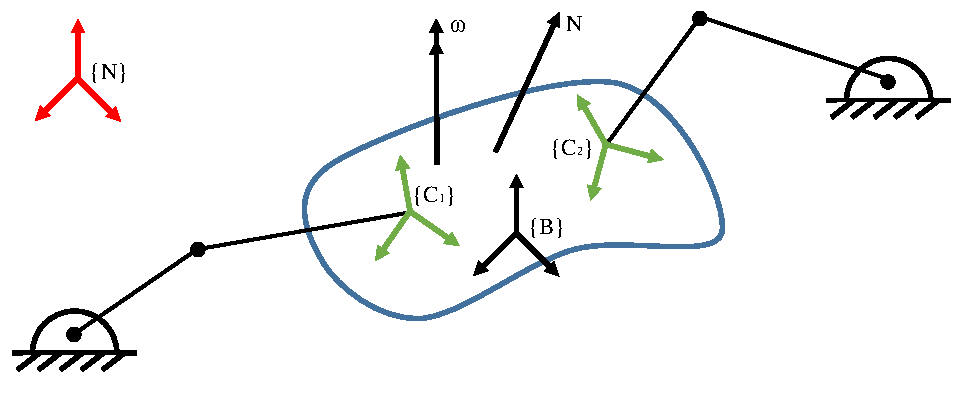
\includegraphics[width=1\textwidth]{figures/GraspingNotationCrop.pdf}
\end{columns}

\end{frame}

%------------------------------------------------

\begin{frame}
\frametitle{Twist and Contacts}
\begin{columns}[c] % The "c" option specifies centered vertical alignment while the "t" option is used for top vertical alignment

\column{.56\textwidth}
In spatial systems (3D), $n_{\nu}$=6, $n_b$=1\\
$\nu = \nu^{N} = \begin{bmatrix}
N_x\\
N_y\\
N_z\\
\omega_x\\
\omega_y\\
\omega_z
\end{bmatrix}, \hspace{.2cm} \nu: twist $

\column{.54\textwidth} 
\centering
 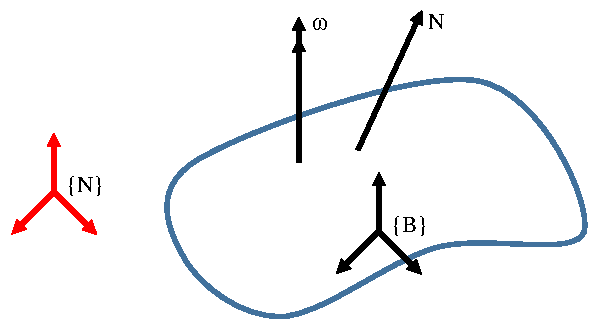
\includegraphics[width=.9\textwidth]{figures/GeneralizedVelocityCrop.pdf}
\end{columns}

\begin{columns}[c] % The "c" option specifies centered vertical alignment while the "t" option is used for top vertical alignment

\column{.56\textwidth}
Two i-$th$ contact points
\begin{itemize}
\item object \vspace{0.2cm}
\item hand \vspace{0.2cm}
\end{itemize}

\column{.54\textwidth} 
\centering
 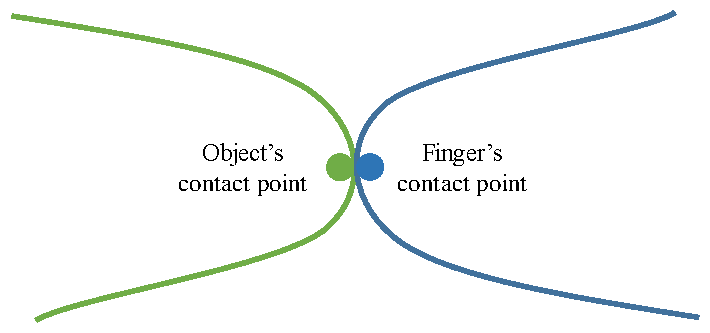
\includegraphics[width=\textwidth]{figures/ContactPointsCrop.pdf}
\end{columns}

\end{frame}

%------------------------------------------------
\subsection{Object Modeling}

\begin{frame}
\frametitle{Twist of Contact on Object}
Goal: Given object's twist $\nu$, compute twist of i-$th$ contact on body 
\begin{equation*}
\nu_{i,obj}^C=\tilde{G}^{\intercal}_i \nu^N,
\end{equation*}
\begin{itemize}
\item $\nu_{i,obj}^C$: twist expressed in frame {$C_i$} \vspace{.2cm}
\item $\nu^N$: twist expressed in inertial frame {$N$} \vspace{.2cm}
\item $\tilde{G}^{\intercal}_i$: partial grasp matrix \vspace{.2cm}
\end{itemize}
\end{frame}

%------------------------------------------------

\begin{frame}
\frametitle{Translational and Angular Velocity }
Object's points have different translational velocity N 
\begin{equation*}
N_{i}^{N}=N^N + \omega^N\times r_{i}^{N} = N^N - r_i^N\times \omega^N= N^N - S(r_i^N) \omega^N,
\end{equation*}
S: Skew-symmetric matrix 
\begin{equation*}
S(a)=\begin{bmatrix}
0 & -a_z & a_y \\
a_z & 0 & -a_x \\
-a_y& a_x & 0 \\
\end{bmatrix}=-S(a)^{\intercal}
\end{equation*}

Angular velocity $\omega$ of all points on an object is the same
\begin{equation*}
\omega^{C_i} = R_{N}^{C_i}\omega^{N}
\end{equation*}

\end{frame}

%------------------------------------------------

\begin{frame}
\frametitle{Rigid Body Equation}
\begin{columns}[c] 
\column{.70\textwidth}

\begin{itemize}
\item Position of contact point i $X^{N}_{i}=X^N + r_{i}$ \vspace{.2cm}
\item Euler theorem: $r_{i} = Rr_{i}^{N}$, with $R^{\intercal}R=I$ \vspace{.2cm}
\item $X^{N}_{i}=X^N + Rr_{i}^{N}$ \vspace{.2cm}
\item $N^{N}_{i}=N^N + \frac{dR}{dt} r_{i}^{N}=N^N + \frac{dR}{dt} R^{\intercal}Rr_{i}^{N}=N^N + \frac{dR}{dt} R^{\intercal}r_{i}= N^N + \Omega r_{i}$ \vspace{.2cm}
\item $\Omega r=\omega\times r $, $\Omega$: angular velocity tensor \vspace{.2cm}
\item $N_{i}^{N}=N^N + \omega^N\times r_{i}^{N}$
\end{itemize}

\column{.40\textwidth} 
\centering
 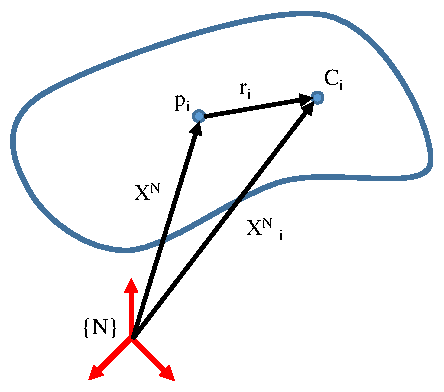
\includegraphics[width=1\textwidth]{figures/RigidBodyCrop.pdf}
\end{columns}
\end{frame}

%------------------------------------------------

\begin{frame}
\frametitle{Twist Transformation to Contact Frame}
The twist results
\begin{equation*}
\begin{bmatrix}
N_{i}^{N}\\
\omega_{i}^{N}
\end{bmatrix}=
\begin{bmatrix}
I_{3x3} & S(r_{i}^{N})^{\intercal}\\
0_{3x3} & I_{3x3} 
\end{bmatrix}
\begin{bmatrix}
N^N\\
\omega^{N}
\end{bmatrix}
\end{equation*}

Vector expression from contact frame ${C_i}$ to inertial frame ${N}$, $d^{N}=R_{C_i}^{N}d^{C_i}\Rightarrow (R_{C_i}^{N})^{\intercal}d^{N}=(R_{C_i}^{N})^{\intercal}R_{C_i}^{N}d^{C_i}\Rightarrow (R_{C_i}^{N})^{\intercal}d^{N}=Id^{C_i} $ \vspace{.2cm}

Thus the twist yields
\begin{equation*}
\nu_{i,obj}=
\begin{bmatrix}
N_{i,obj}^{C_i}\\
\omega_{i,obj}^{C_i}
\end{bmatrix}=
\begin{bmatrix}
(R_{C_i}^{N})^{\intercal} & 0\\
0 &(R_{C_i}^{N})^{\intercal} 
\end{bmatrix}
\begin{bmatrix}
I & S(r_{i}^{N})^{\intercal}\\
0 & I
\end{bmatrix}
\begin{bmatrix}
N^N\\
\omega^{N}
\end{bmatrix}=\tilde{G}^{\intercal}_i \nu^N
\end{equation*}
\end{frame}

%------------------------------------------------
\subsection{Hand Modeling}

\begin{frame}
\frametitle{Twist of Contact in Hand}
Goal: Given joint angles $\dot{q}$, compute twist of i-$th$ contact in hand 
\begin{equation*}
\nu_{i,hand}^C=\tilde{J}_i \dot{q},
\end{equation*}
\begin{itemize}
\item $\nu_{i,hand}^C$: twist expressed in frame {$C_i$} \vspace{.2cm}
\item $\dot{q}$: joint angles \vspace{.2cm}
\item $\tilde{J}_i$: partial hand Jacobian matrix \vspace{.2cm}
\end{itemize}
\end{frame}

%------------------------------------------------

\begin{frame}
\frametitle{Translational Velocity }
Hand's translational N, similar w/ Jacobian in velocity kinematics 
\begin{equation*}
N_{ij}=d_{ij}^N\dot{q}=\begin{bmatrix}
0\\
\hat{z}_{j}^{N}\dot{q}_j\\
\hat{z}_{j}^{N}\dot{q}_j\times (C_{i}^{N}-\zeta_{j}^{N})
\end{bmatrix}
\begin{matrix}
\rightarrow no \hspace{.1cm} contact\\
\rightarrow prismatic \hspace{.1cm} joint\\
\rightarrow revolute \hspace{.1cm} joint
\end{matrix}
\end{equation*}
Revolute joint can be written 
$\hat{z}_{j}^{N}\dot{q}_j\times (C_{i}^{N}-\zeta_{j}^{N})=-(C_{i}^{N}-\zeta_{j}^{N})\times \hat{z}_{j}^{N}\dot{q}_j=S^{\intercal}(C_{i}^{N}-\zeta_{j}^{N})\hat{z}_{j}^{N}\dot{q}_j$

\begin{columns}[c] 
\column{.50\textwidth}
\begin{itemize}
\item $\zeta_j$: origin of joint frame
\item j: joint 
\end{itemize}

\column{.50\textwidth}
\centering
 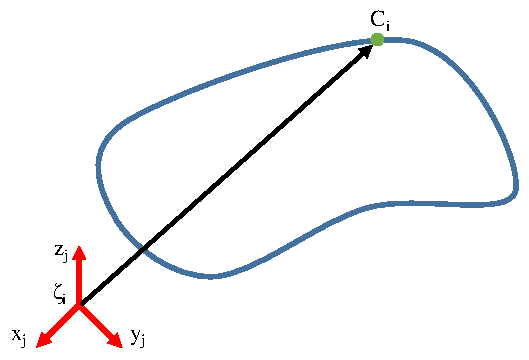
\includegraphics[width=.8\textwidth]{figures/HandTranslationCrop.pdf}
\end{columns}

\end{frame}
%------------------------------------------------

\begin{frame}
\frametitle{Angular Velocity and Finger Contacts}
Angular velocity $\omega_{ij}^{N}=l_{ij}^{N}\dot{q}_{ij}$,
\begin{equation*}
l_{ij}=\begin{bmatrix}
0\\
0\\
\hat{z}_{j}^{N}
\end{bmatrix}
\begin{matrix}
\rightarrow no \hspace{.1cm} contact\\
\rightarrow prismatic \hspace{.1cm} joint\\
\rightarrow revolute \hspace{.1cm} joint
\end{matrix}
\end{equation*}
which yields 
\begin{equation*}
\nu_{ij}^N= \begin{bmatrix}
d_{ij}^N\\
l_{ij}^N
\end{bmatrix}\dot{q}_i
\end{equation*}
For all finger contacts
\begin{equation*}
\nu_{i,hand}^N= \begin{bmatrix}
d_{i,1}^N \cdots d_{i,n_q}^N\\
l_{i,1}^N \cdots l_{i,n_q}^N
\end{bmatrix}\begin{bmatrix}
\dot{q}_1\\
\vdots \\
\dot{q}_{n_q}
\end{bmatrix}=Z_i\dot{q}
\end{equation*}


\end{frame}
%------------------------------------------------

\begin{frame}
\frametitle{Partial Hand Jacobian}
\begin{itemize}
\item Transfrom twist to contact frame
\begin{equation*}
\nu_{i,hand}^C=\overline{R}_{i}^{\intercal} Z_i\dot{q}=\tilde{J}_i \dot{q}, \hspace{.2cm} \tilde{J}_i \in \mathbb{R}^{6n_c\times n_q}
\end{equation*}
\vspace{.2cm}
\item Partial hand Jacobian $\tilde{J}_i$, maps joint velocities with the contact twists of the hand
\end{itemize}

\end{frame}

%------------------------------------------------

\begin{frame}
\frametitle{Complete Hand Jacobian and Grasp Matrix}
For all contacts we get
\begin{equation*}
\nu_{C,hand}=\begin{bmatrix}
\nu_{1,hand}\\
\vdots\\
\nu_{n_c,hand}
\end{bmatrix}, \hspace{.2cm} \nu_{C,obj}=\begin{bmatrix}
\nu_{1,obj}\\
\vdots\\
\nu_{n_c,obj}
\end{bmatrix}
\end{equation*}
Complete hand Jacobian and grasp matrix
\begin{equation*}
\tilde{J}=\begin{bmatrix}
\tilde{J}_{1}\\
\vdots\\
\tilde{J}_{n_c}
\end{bmatrix}, \hspace{.2cm} \tilde{G}^{\intercal}=\begin{bmatrix}
\tilde{G}^{\intercal}_{1}\\
\vdots\\
\tilde{G}^{\intercal}_{n_c}
\end{bmatrix}
\end{equation*}


\end{frame}

%----------------------------------------------
\subsection{Contact Modeling}
\begin{frame}
\frametitle{Models of interest}
Three models of interest
\begin{itemize}
\item Point contact w/o friction (PwoF)
\item Hard finger (HF)
\item Soft finger (SF)
\end{itemize}
\vspace{.2cm}
Relative twist at i-$th$ contact
\begin{equation*}
(\tilde{J}_{i}-\tilde{G}_{i}^{\intercal})\begin{pmatrix}
\dot{q}\\
\nu
\end{pmatrix}=(\nu_{i,hand} - \nu_{i,obj})
\end{equation*}
\vspace{.2cm}
Particular contact model through homogeneous $H_i\in \mathbb{R}^{l_i\times 6}$
\begin{equation*}
H_i(\nu_{i,hand} - \nu_{i,obj})=0
\end{equation*}

\end{frame}

%----------------------------------------------

\begin{frame}
\frametitle{Homogeneous matrix}
\begin{itemize}
\item Homogeneous matrix defined as
\begin{equation*}
H_i= \begin{bmatrix}
H_{iF} & 0\\
0 & H_{iM}
\end{bmatrix}, 
\end{equation*}
$H_{iF}$: Translational components \\
$H_{iM}$: Rotational components
\item Contact models matrices selection
\begin{table}
%\centering
\begin{tabular}{|c|c|c|c|}
\hline \scriptsize{Model} &  \scriptsize{$l_i$} & \scriptsize{$H_{iF}$} & \scriptsize{$H_{iM}$} \\
\hline \scriptsize{PwoF} & \scriptsize{1}  & \scriptsize{(1 0 0)} & \scriptsize{0} \\
\hline \scriptsize{HF} & \scriptsize{3}  & \scriptsize{$I_{3x3}$} & \scriptsize{0}  \\
\hline \scriptsize{SF} & \scriptsize{4} & \scriptsize{$I_{3x3}$} & \scriptsize{(1 0 0)} \\
\hline
\end{tabular}
\end{table}
$l_i$: transmitted twist components 
\end{itemize}

\end{frame}

%----------------------------------------------

\begin{frame}
\frametitle{Hand Jacobian and Grasp Matrix}
\begin{itemize}
\item From the complete hand Jacobian and grasp matrix we get
\begin{equation*}
H(\nu_{C,hand} - \nu_{C,obj})=H(\tilde{J}\dot{q} -\tilde{G}^{\intercal}\nu)=(H\tilde{J}-H\tilde{G}^{\intercal})\begin{pmatrix}
\dot{q}\\
\nu
\end{pmatrix}=0
\end{equation*}
\item Hand Jacobian and grasp matrix are
\begin{equation*}
J\dot{q}=\nu_{cc,obj}=\nu_{cc,hand}=G^{\intercal}\nu
\end{equation*}
$J=H\tilde{J}$, hand Jacobian matrix\\
$G^{\intercal}=H\tilde{G}^{\intercal}$, grasp matrix\\
\end{itemize}

\end{frame}

%----------------------------------------------

\subsection{Conclusions}
\begin{frame}
\frametitle{Conclusions}
Robot grasping procedure
\begin{itemize}
\item Given: Contact points $C_i$, hand kinematic structure, object velocity twists $\nu$, and joint velocities $\dot{q}$ 
\item Compute: Velocities of contact points on objects $\nu_{C,hand}$, and velocities of contact points in hand $\nu_{C,onj}$ \vspace{0.2cm}
\item Given: Contact model 
\item Compute: Hand Jacobian matrix, Grasp matrix \vspace{0.2cm}
\end{itemize}
\end{frame}
%----------------------------------------------


%------------------------------------------------
\section{References}
%------------------------------------------------

\begin{frame}
\frametitle{References}
\footnotesize{
\begin{thebibliography}{99}

\bibitem[Prattichizzo, 2016]{p1} D.Prattichizzo and J.Trinkle (2016)
\newblock Grasping
\newblock \emph{Springer handbook of robotics, 955--988}, 2016.

\end{thebibliography}
}
\end{frame}

%------------------------------------------------
\section{}
\begin{frame}
\begin{center}
\Huge {Thank You!}
\end{center}
\end{frame}

%----------------------------------------------------------------------------------------

\end{document} 